%%%%%%%%%%%%%%%%%%%%%%%%%%%%%%%%%%%%%%%%%%%%%%%%%%%%%%%%%%%%%%%%%%%%%%%%%%%%%%%
% Chapter 'Refrigerants - Water'
%%%%%%%%%%%%%%%%%%%%%%%%%%%%%%%%%%%%%%%%%%%%%%%%%%%%%%%%%%%%%%%%%%%%%%%%%%%%%%%
\section{Water}
%
%%%%%%%%%%%%%%%%%%%%%%%%%%%%%%%%%%%%%%%%%%%%%%%%%%%%%%%%%%%%%%%%%%%%%%%%%%%%%%%
%%%%%%%%%%%%%%%%%%%%%%%%%%%%%%%%%%%%%%%%%%%%%%%%%%%%%%%%%%%%%%%%%%%%%%%%%%%%%%%
\subsection{Saturated Liquid Density - EoS1 - ID 1}
%
\begin{tabular}[l]{|lp{11.5cm}|}
\hline
\addlinespace

\textbf{Name:} & Water \\
\textbf{Equation:} & SaturatedLiquidDensity\_EoS1 \\
\textbf{ID:} & 1 \\
\textbf{Reference:} & Wagner, W.; Pruß, A. (2002): The IAPWS Formulation 1995 for the Thermodynamic Properties of Ordinary Water Substance for General and Scientific Use. In: Journal of Physical and Chemical Reference Data 31 (2), S. 387–535. DOI: 10.1063/1.1461829. \\
\textbf{Comment:} & None \\

\addlinespace
\hline
\end{tabular}
\newline

\textbf{Equation and parameters:}
\newline
%
Saturated liquid density $\rho_\mathrm{sat}^\mathrm{liq}$ in $\si{\kilogram\per\cubic\meter}$ is calculated depending on temperature $T$ in $\si{\kelvin}$ by:
%
\begin{equation*}
\begin{split}
\rho_\mathrm{sat}^\mathrm{liq} &=& \begin{cases} \rho_\mathrm{ref} \exp(\Omega) & \quad \text{if flag } < 0 \\ \rho_\mathrm{ref} \Omega & \quad \text{else} \end{cases} & \quad\text{, with} \\
\Omega &=& \sum_{i=1}^{8} a_i \xi^{b_i} & \quad\text{, and} \\
\xi &=& 1 - \theta & \quad\text{, and} \\
\theta &=& \nicefrac{T}{T_\mathrm{crit}} & \quad\text{.}
\end{split}
\end{equation*}
%
The parameters of the equation are:
%
\begin{longtable}[l]{lll|lll}
\toprule
\addlinespace
\textbf{Par.} & \textbf{Unit} & \textbf{Value} &	\textbf{Par.} & \textbf{Unit} & \textbf{Value} \\
\addlinespace
\midrule
\endhead

\bottomrule
\endfoot
\bottomrule
\endlastfoot
\addlinespace

flag & - & 1.000000000e+00 & $b_4$ & - & 1.666666667e+00 \\
$T_\mathrm{crit}$ & $\si{\kelvin}$ & 6.470960000e+02 & $a_5$ & - & -1.754934790e+00 \\
$\rho_\mathrm{ref}$ & $\si{\kilogram\per\cubic\meter}$ & 3.220000000e+02 & $b_5$ & - & 5.333333333e+00 \\
$a_1$ & - & 1.000000000e+00 & $a_6$ & - & -4.551703520e+01 \\
$b_1$ & - & 0.000000000e+00 & $b_6$ & - & 1.433333333e+01 \\
$a_2$ & - & 1.992740640e+00 & $a_7$ & - & -6.746944500e+05 \\
$b_2$ & - & 3.333333333e-01 & $b_7$ & - & 3.666666667e+01 \\
$a_3$ & - & 1.099653420e+00 & $a_8$ & - & 0.000000000e+00 \\
$b_3$ & - & 6.666666667e-01 & $b_8$ & - & 0.000000000e+00 \\
$a_4$ & - & -5.108393030e-01 & & & \\

\addlinespace\end{longtable}

\textbf{Validity:}
\newline
Equation is approximately valid for $273.16 \si{\kelvin} \leq T \leq 647.096 \si{\kelvin}$.
\newline

\textbf{Visualization:}
%
\begin{figure}[!htp]
{\noindent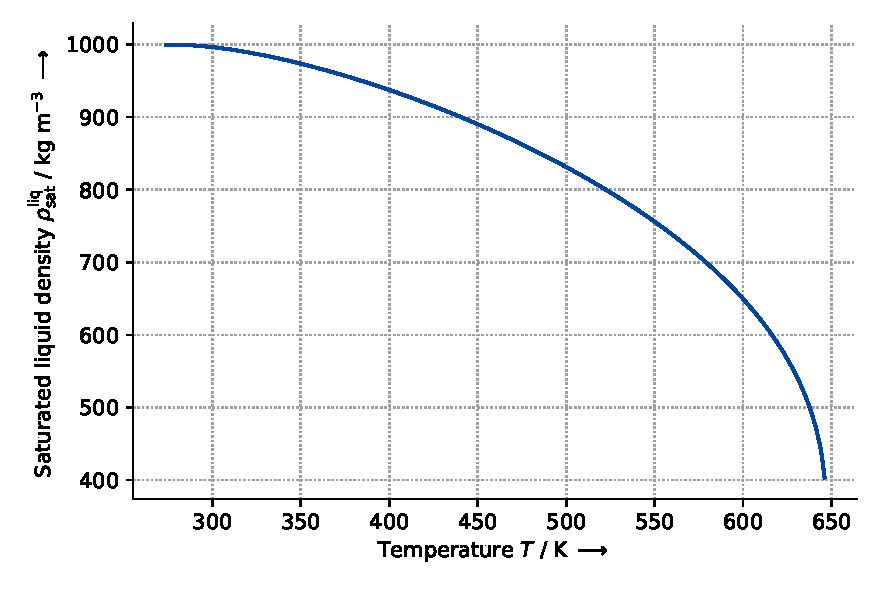
\includegraphics[height=10cm, keepaspectratio]{figs/ref/ref_Water_SaturatedLiquidDensity_EoS1_1.pdf}}
\end{figure}
%

\FloatBarrier
\newpage
%%%%%%%%%%%%%%%%%%%%%%%%%%%%%%%%%%%%%%%%%%%%%%%%%%%%%%%%%%%%%%%%%%%%%%%%%%%%%%%
%%%%%%%%%%%%%%%%%%%%%%%%%%%%%%%%%%%%%%%%%%%%%%%%%%%%%%%%%%%%%%%%%%%%%%%%%%%%%%%
\subsection{Saturated Liquid Density - EoS1 - ID 2}
%
\begin{tabular}[l]{|lp{11.5cm}|}
\hline
\addlinespace

\textbf{Name:} & Water \\
\textbf{Equation:} & SaturatedLiquidDensity\_EoS1 \\
\textbf{ID:} & 2 \\
\textbf{Reference:} & Verein Deutscher Ingenieure (2010): VDI Heat Atlas. 2. Ed. Heidelberg: Springer. Online: http://dx.doi.org/10.1007/978-3-540-77877-6. \\
\textbf{Comment:} & None \\

\addlinespace
\hline
\end{tabular}
\newline

\textbf{Equation and parameters:}
\newline
%
Saturated liquid density $\rho_\mathrm{sat}^\mathrm{liq}$ in $\si{\kilogram\per\cubic\meter}$ is calculated depending on temperature $T$ in $\si{\kelvin}$ by:
%
\begin{equation*}
\begin{split}
\rho_\mathrm{sat}^\mathrm{liq} &=& \begin{cases} \rho_\mathrm{ref} \exp(\Omega) & \quad \text{if flag } < 0 \\ \rho_\mathrm{ref} \Omega & \quad \text{else} \end{cases} & \quad\text{, with} \\
\Omega &=& \sum_{i=1}^{8} a_i \xi^{b_i} & \quad\text{, and} \\
\xi &=& 1 - \theta & \quad\text{, and} \\
\theta &=& \nicefrac{T}{T_\mathrm{crit}} & \quad\text{.}
\end{split}
\end{equation*}
%
The parameters of the equation are:
%
\begin{longtable}[l]{lll|lll}
\toprule
\addlinespace
\textbf{Par.} & \textbf{Unit} & \textbf{Value} &	\textbf{Par.} & \textbf{Unit} & \textbf{Value} \\
\addlinespace
\midrule
\endhead

\bottomrule
\endfoot
\bottomrule
\endlastfoot
\addlinespace

flag & - & 1.000000000e+00 & $b_4$ & - & 1.000000000e+00 \\
$T_\mathrm{crit}$ & $\si{\kelvin}$ & 6.471000000e+02 & $a_5$ & - & -7.701282609e+00 \\
$\rho_\mathrm{ref}$ & $\si{\kilogram\per\cubic\meter}$ & 3.220000000e+02 & $b_5$ & - & 1.333333333e+00 \\
$a_1$ & - & 1.000000000e+00 & $a_6$ & - & 0.000000000e+00 \\
$b_1$ & - & 0.000000000e+00 & $b_6$ & - & 0.000000000e+00 \\
$a_2$ & - & 3.397587888e+00 & $a_7$ & - & 0.000000000e+00 \\
$b_2$ & - & 3.500000000e-01 & $b_7$ & - & 0.000000000e+00 \\
$a_3$ & - & -5.631147516e+00 & $a_8$ & - & 0.000000000e+00 \\
$b_3$ & - & 6.666666667e-01 & $b_8$ & - & 0.000000000e+00 \\
$a_4$ & - & 1.199986242e+01 & & & \\

\addlinespace\end{longtable}

\textbf{Validity:}
\newline
Equation is approximately valid for $273.16 \si{\kelvin} \leq T \leq 647.1 \si{\kelvin}$.
\newline

\textbf{Visualization:}
%
\begin{figure}[!htp]
{\noindent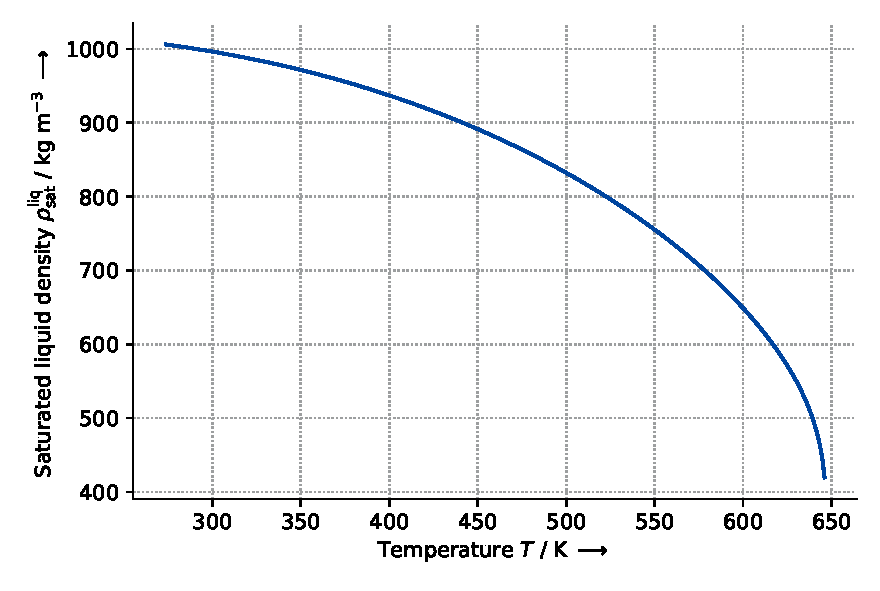
\includegraphics[height=10cm, keepaspectratio]{figs/ref/ref_Water_SaturatedLiquidDensity_EoS1_2.pdf}}
\end{figure}
%

\FloatBarrier
\newpage
%%%%%%%%%%%%%%%%%%%%%%%%%%%%%%%%%%%%%%%%%%%%%%%%%%%%%%%%%%%%%%%%%%%%%%%%%%%%%%%
%%%%%%%%%%%%%%%%%%%%%%%%%%%%%%%%%%%%%%%%%%%%%%%%%%%%%%%%%%%%%%%%%%%%%%%%%%%%%%%
\subsection{Vapor Pressure - Antoine - ID 1}
%
\begin{tabular}[l]{|lp{11.5cm}|}
\hline
\addlinespace

\textbf{Name:} & Water \\
\textbf{Equation:} & VaporPressure\_Antoine \\
\textbf{ID:} & 1 \\
\textbf{Reference:} & P.J. Linstrom and W.G. Mallard, Eds., NIST Chemistry WebBook, NIST Standard Reference Database Number 69, National Institute of Standards and Technology, Gaithersburg MD, 20899, https://doi.org/10.18434/T4D303. \\
\textbf{Comment:} & None \\

\addlinespace
\hline
\end{tabular}
\newline

\textbf{Equation and parameters:}
\newline
%
Vapor pressure $p_\mathrm{sat}$ in $\si{\pascal}$ is calculated depending on temperature $T$ in $\si{\kelvin}$ by:
%
\begin{equation*}
\nicefrac{p_\mathrm{sat}}{100000} = 10^{a - \nicefrac{b}{T + c}}
\end{equation*}
%
The parameters of the equation are:
%
\begin{longtable}[l]{lll|lll}
\toprule
\addlinespace
\textbf{Par.} & \textbf{Unit} & \textbf{Value} &	\textbf{Par.} & \textbf{Unit} & \textbf{Value} \\
\addlinespace
\midrule
\endhead

\bottomrule
\endfoot
\bottomrule
\endlastfoot
\addlinespace

$a$ & - & 3.559590000e+00 & $c$ & $\si{\kelvin}$  & -1.980430000e+02 \\
$b$ & $\si{\kelvin}$ & 6.437480000e+02 & & & \\

\addlinespace\end{longtable}

\textbf{Validity:}
\newline
Equation is approximately valid for $379.0 \si{\kelvin} \leq T \leq 583.0 \si{\kelvin}$.
\newline

\textbf{Visualization:}
%
\begin{figure}[!htp]
{\noindent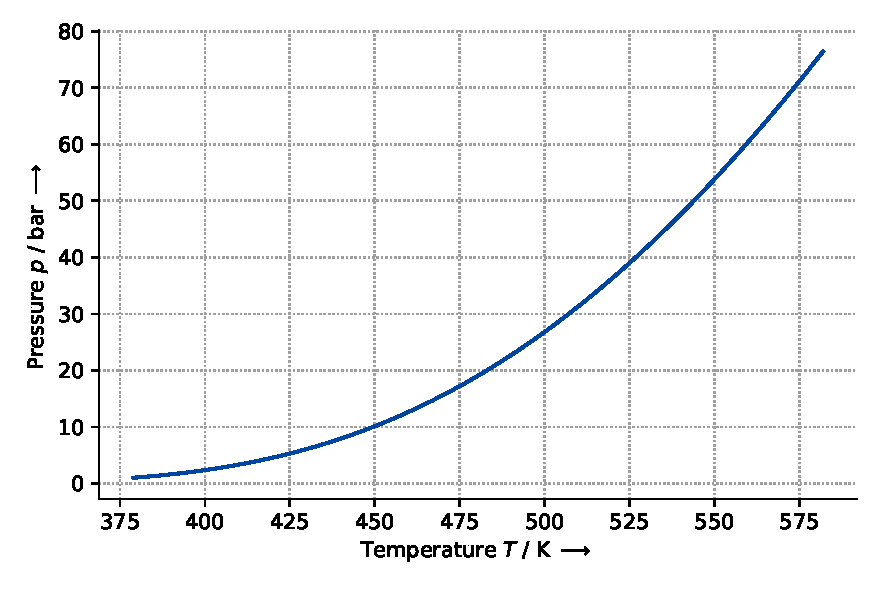
\includegraphics[height=10cm, keepaspectratio]{figs/ref/ref_Water_VaporPressure_Antoine_1.pdf}}
\end{figure}
%

\FloatBarrier
\newpage
%%%%%%%%%%%%%%%%%%%%%%%%%%%%%%%%%%%%%%%%%%%%%%%%%%%%%%%%%%%%%%%%%%%%%%%%%%%%%%%
%%%%%%%%%%%%%%%%%%%%%%%%%%%%%%%%%%%%%%%%%%%%%%%%%%%%%%%%%%%%%%%%%%%%%%%%%%%%%%%
\subsection{Vapor Pressure - Antoine - ID 2}
%
\begin{tabular}[l]{|lp{11.5cm}|}
\hline
\addlinespace

\textbf{Name:} & Water \\
\textbf{Equation:} & VaporPressure\_Antoine \\
\textbf{ID:} & 2 \\
\textbf{Reference:} & P.J. Linstrom and W.G. Mallard, Eds., NIST Chemistry WebBook, NIST Standard Reference Database Number 69, National Institute of Standards and Technology, Gaithersburg MD, 20899, https://doi.org/10.18434/T4D303. \\
\textbf{Comment:} & None \\

\addlinespace
\hline
\end{tabular}
\newline

\textbf{Equation and parameters:}
\newline
%
Vapor pressure $p_\mathrm{sat}$ in $\si{\pascal}$ is calculated depending on temperature $T$ in $\si{\kelvin}$ by:
%
\begin{equation*}
\nicefrac{p_\mathrm{sat}}{100000} = 10^{a - \nicefrac{b}{T + c}}
\end{equation*}
%
The parameters of the equation are:
%
\begin{longtable}[l]{lll|lll}
\toprule
\addlinespace
\textbf{Par.} & \textbf{Unit} & \textbf{Value} &	\textbf{Par.} & \textbf{Unit} & \textbf{Value} \\
\addlinespace
\midrule
\endhead

\bottomrule
\endfoot
\bottomrule
\endlastfoot
\addlinespace

$a$ & - & 5.402210000e+00 & $c$ & $\si{\kelvin}$  & -3.173700000e+01 \\
$b$ & $\si{\kelvin}$ & 1.838675000e+03 & & & \\

\addlinespace\end{longtable}

\textbf{Validity:}
\newline
Equation is approximately valid for $273.0 \si{\kelvin} \leq T \leq 303.0 \si{\kelvin}$.
\newline

\textbf{Visualization:}
%
\begin{figure}[!htp]
{\noindent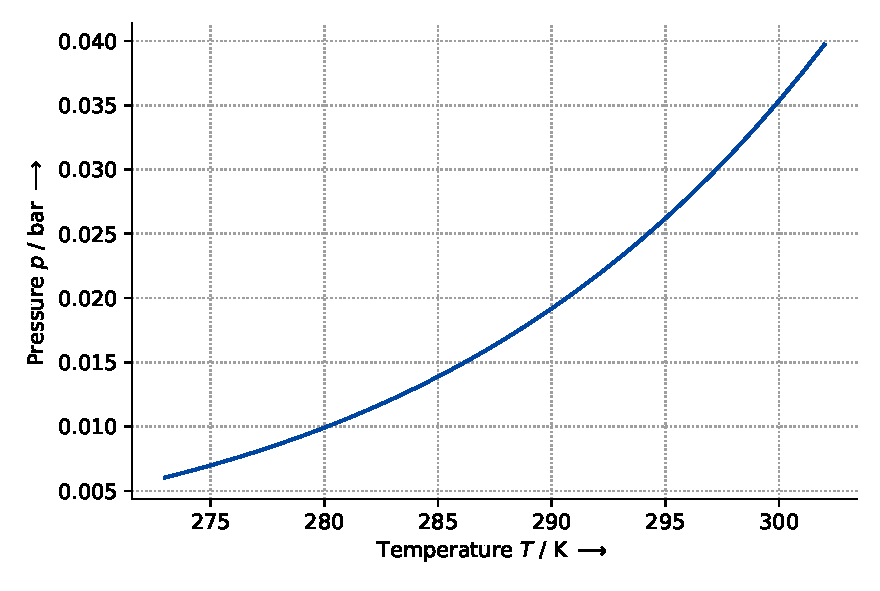
\includegraphics[height=10cm, keepaspectratio]{figs/ref/ref_Water_VaporPressure_Antoine_2.pdf}}
\end{figure}
%

\FloatBarrier
\newpage
%%%%%%%%%%%%%%%%%%%%%%%%%%%%%%%%%%%%%%%%%%%%%%%%%%%%%%%%%%%%%%%%%%%%%%%%%%%%%%%
%%%%%%%%%%%%%%%%%%%%%%%%%%%%%%%%%%%%%%%%%%%%%%%%%%%%%%%%%%%%%%%%%%%%%%%%%%%%%%%
\subsection{Vapor Pressure - Antoine - ID 3}
%
\begin{tabular}[l]{|lp{11.5cm}|}
\hline
\addlinespace

\textbf{Name:} & Water \\
\textbf{Equation:} & VaporPressure\_Antoine \\
\textbf{ID:} & 3 \\
\textbf{Reference:} & P.J. Linstrom and W.G. Mallard, Eds., NIST Chemistry WebBook, NIST Standard Reference Database Number 69, National Institute of Standards and Technology, Gaithersburg MD, 20899, https://doi.org/10.18434/T4D303. \\
\textbf{Comment:} & None \\

\addlinespace
\hline
\end{tabular}
\newline

\textbf{Equation and parameters:}
\newline
%
Vapor pressure $p_\mathrm{sat}$ in $\si{\pascal}$ is calculated depending on temperature $T$ in $\si{\kelvin}$ by:
%
\begin{equation*}
\nicefrac{p_\mathrm{sat}}{100000} = 10^{a - \nicefrac{b}{T + c}}
\end{equation*}
%
The parameters of the equation are:
%
\begin{longtable}[l]{lll|lll}
\toprule
\addlinespace
\textbf{Par.} & \textbf{Unit} & \textbf{Value} &	\textbf{Par.} & \textbf{Unit} & \textbf{Value} \\
\addlinespace
\midrule
\endhead

\bottomrule
\endfoot
\bottomrule
\endlastfoot
\addlinespace

$a$ & - & 5.203890000e+00 & $c$ & $\si{\kelvin}$  & -3.948500000e+01 \\
$b$ & $\si{\kelvin}$ & 1.733926000e+03 & & & \\

\addlinespace\end{longtable}

\textbf{Validity:}
\newline
Equation is approximately valid for $304.0 \si{\kelvin} \leq T \leq 333.0 \si{\kelvin}$.
\newline

\textbf{Visualization:}
%
\begin{figure}[!htp]
{\noindent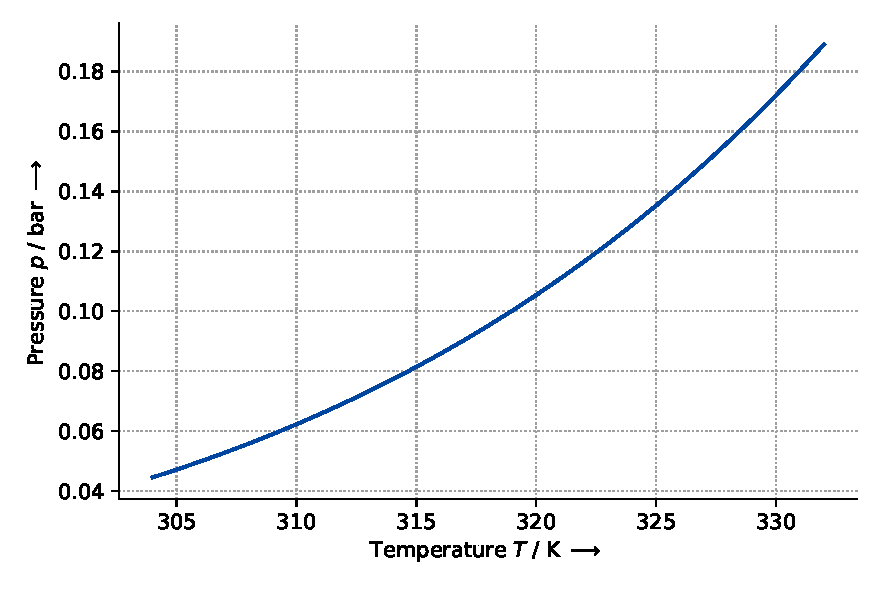
\includegraphics[height=10cm, keepaspectratio]{figs/ref/ref_Water_VaporPressure_Antoine_3.pdf}}
\end{figure}
%

\FloatBarrier
\newpage
%%%%%%%%%%%%%%%%%%%%%%%%%%%%%%%%%%%%%%%%%%%%%%%%%%%%%%%%%%%%%%%%%%%%%%%%%%%%%%%
%%%%%%%%%%%%%%%%%%%%%%%%%%%%%%%%%%%%%%%%%%%%%%%%%%%%%%%%%%%%%%%%%%%%%%%%%%%%%%%
\subsection{Vapor Pressure - Antoine - ID 4}
%
\begin{tabular}[l]{|lp{11.5cm}|}
\hline
\addlinespace

\textbf{Name:} & Water \\
\textbf{Equation:} & VaporPressure\_Antoine \\
\textbf{ID:} & 4 \\
\textbf{Reference:} & P.J. Linstrom and W.G. Mallard, Eds., NIST Chemistry WebBook, NIST Standard Reference Database Number 69, National Institute of Standards and Technology, Gaithersburg MD, 20899, https://doi.org/10.18434/T4D303. \\
\textbf{Comment:} & None \\

\addlinespace
\hline
\end{tabular}
\newline

\textbf{Equation and parameters:}
\newline
%
Vapor pressure $p_\mathrm{sat}$ in $\si{\pascal}$ is calculated depending on temperature $T$ in $\si{\kelvin}$ by:
%
\begin{equation*}
\nicefrac{p_\mathrm{sat}}{100000} = 10^{a - \nicefrac{b}{T + c}}
\end{equation*}
%
The parameters of the equation are:
%
\begin{longtable}[l]{lll|lll}
\toprule
\addlinespace
\textbf{Par.} & \textbf{Unit} & \textbf{Value} &	\textbf{Par.} & \textbf{Unit} & \textbf{Value} \\
\addlinespace
\midrule
\endhead

\bottomrule
\endfoot
\bottomrule
\endlastfoot
\addlinespace

$a$ & - & 5.076800000e+00 & $c$ & $\si{\kelvin}$  & -4.585400000e+01 \\
$b$ & $\si{\kelvin}$ & 1.659793000e+03 & & & \\

\addlinespace\end{longtable}

\textbf{Validity:}
\newline
Equation is approximately valid for $334.0 \si{\kelvin} \leq T \leq 363.0 \si{\kelvin}$.
\newline

\textbf{Visualization:}
%
\begin{figure}[!htp]
{\noindent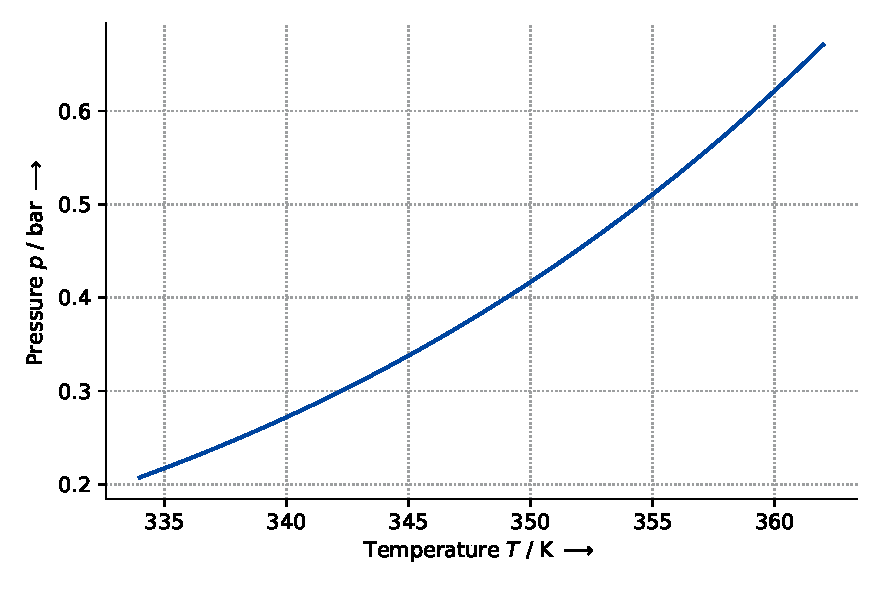
\includegraphics[height=10cm, keepaspectratio]{figs/ref/ref_Water_VaporPressure_Antoine_4.pdf}}
\end{figure}
%

\FloatBarrier
\newpage
%%%%%%%%%%%%%%%%%%%%%%%%%%%%%%%%%%%%%%%%%%%%%%%%%%%%%%%%%%%%%%%%%%%%%%%%%%%%%%%
%%%%%%%%%%%%%%%%%%%%%%%%%%%%%%%%%%%%%%%%%%%%%%%%%%%%%%%%%%%%%%%%%%%%%%%%%%%%%%%
\subsection{Vapor Pressure - Antoine - ID 5}
%
\begin{tabular}[l]{|lp{11.5cm}|}
\hline
\addlinespace

\textbf{Name:} & Water \\
\textbf{Equation:} & VaporPressure\_Antoine \\
\textbf{ID:} & 5 \\
\textbf{Reference:} & P.J. Linstrom and W.G. Mallard, Eds., NIST Chemistry WebBook, NIST Standard Reference Database Number 69, National Institute of Standards and Technology, Gaithersburg MD, 20899, https://doi.org/10.18434/T4D303. \\
\textbf{Comment:} & None \\

\addlinespace
\hline
\end{tabular}
\newline

\textbf{Equation and parameters:}
\newline
%
Vapor pressure $p_\mathrm{sat}$ in $\si{\pascal}$ is calculated depending on temperature $T$ in $\si{\kelvin}$ by:
%
\begin{equation*}
\nicefrac{p_\mathrm{sat}}{100000} = 10^{a - \nicefrac{b}{T + c}}
\end{equation*}
%
The parameters of the equation are:
%
\begin{longtable}[l]{lll|lll}
\toprule
\addlinespace
\textbf{Par.} & \textbf{Unit} & \textbf{Value} &	\textbf{Par.} & \textbf{Unit} & \textbf{Value} \\
\addlinespace
\midrule
\endhead

\bottomrule
\endfoot
\bottomrule
\endlastfoot
\addlinespace

$a$ & - & 5.083540000e+00 & $c$ & $\si{\kelvin}$  & -4.562200000e+01 \\
$b$ & $\si{\kelvin}$ & 1.663125000e+03 & & & \\

\addlinespace\end{longtable}

\textbf{Validity:}
\newline
Equation is approximately valid for $344.0 \si{\kelvin} \leq T \leq 373.0 \si{\kelvin}$.
\newline

\textbf{Visualization:}
%
\begin{figure}[!htp]
{\noindent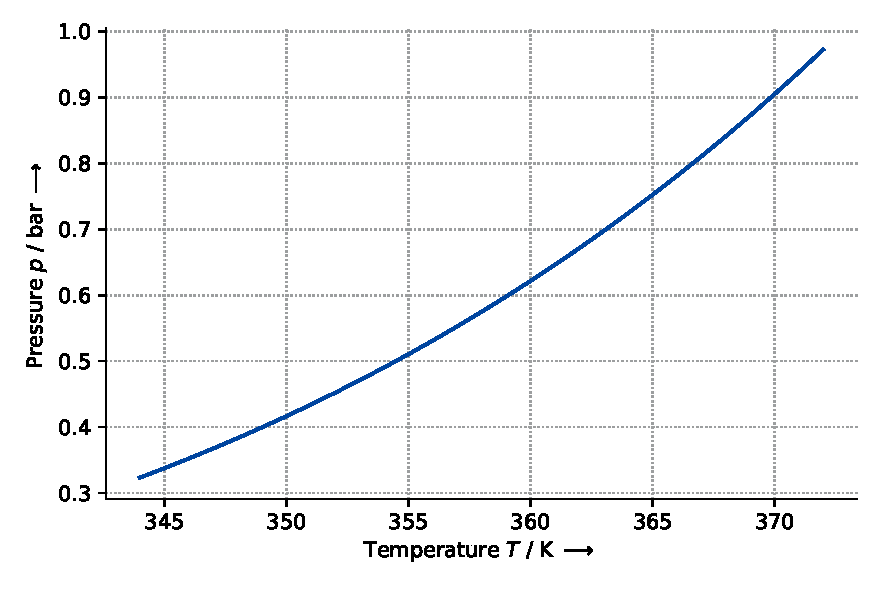
\includegraphics[height=10cm, keepaspectratio]{figs/ref/ref_Water_VaporPressure_Antoine_5.pdf}}
\end{figure}
%

\FloatBarrier
\newpage
%%%%%%%%%%%%%%%%%%%%%%%%%%%%%%%%%%%%%%%%%%%%%%%%%%%%%%%%%%%%%%%%%%%%%%%%%%%%%%%
%%%%%%%%%%%%%%%%%%%%%%%%%%%%%%%%%%%%%%%%%%%%%%%%%%%%%%%%%%%%%%%%%%%%%%%%%%%%%%%
\subsection{Vapor Pressure - Antoine - ID 6}
%
\begin{tabular}[l]{|lp{11.5cm}|}
\hline
\addlinespace

\textbf{Name:} & Water \\
\textbf{Equation:} & VaporPressure\_Antoine \\
\textbf{ID:} & 6 \\
\textbf{Reference:} & P.J. Linstrom and W.G. Mallard, Eds., NIST Chemistry WebBook, NIST Standard Reference Database Number 69, National Institute of Standards and Technology, Gaithersburg MD, 20899, https://doi.org/10.18434/T4D303. \\
\textbf{Comment:} & None \\

\addlinespace
\hline
\end{tabular}
\newline

\textbf{Equation and parameters:}
\newline
%
Vapor pressure $p_\mathrm{sat}$ in $\si{\pascal}$ is calculated depending on temperature $T$ in $\si{\kelvin}$ by:
%
\begin{equation*}
\nicefrac{p_\mathrm{sat}}{100000} = 10^{a - \nicefrac{b}{T + c}}
\end{equation*}
%
The parameters of the equation are:
%
\begin{longtable}[l]{lll|lll}
\toprule
\addlinespace
\textbf{Par.} & \textbf{Unit} & \textbf{Value} &	\textbf{Par.} & \textbf{Unit} & \textbf{Value} \\
\addlinespace
\midrule
\endhead

\bottomrule
\endfoot
\bottomrule
\endlastfoot
\addlinespace

$a$ & - & 6.209630000e+00 & $c$ & $\si{\kelvin}$  & 7.559000000e+00 \\
$b$ & $\si{\kelvin}$ & 2.354731000e+03 & & & \\

\addlinespace\end{longtable}

\textbf{Validity:}
\newline
Equation is approximately valid for $293.0 \si{\kelvin} \leq T \leq 343.0 \si{\kelvin}$.
\newline

\textbf{Visualization:}
%
\begin{figure}[!htp]
{\noindent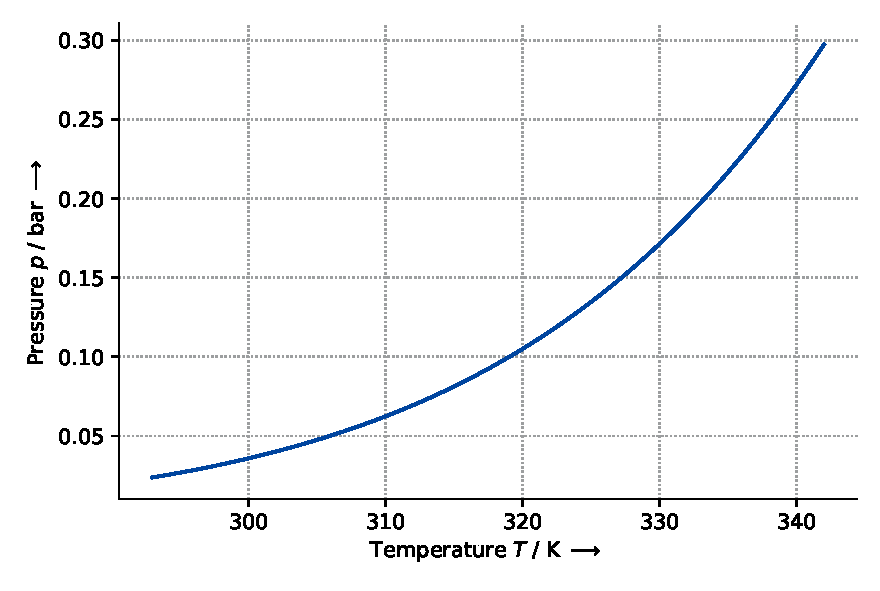
\includegraphics[height=10cm, keepaspectratio]{figs/ref/ref_Water_VaporPressure_Antoine_6.pdf}}
\end{figure}
%

\FloatBarrier
\newpage
%%%%%%%%%%%%%%%%%%%%%%%%%%%%%%%%%%%%%%%%%%%%%%%%%%%%%%%%%%%%%%%%%%%%%%%%%%%%%%%
%%%%%%%%%%%%%%%%%%%%%%%%%%%%%%%%%%%%%%%%%%%%%%%%%%%%%%%%%%%%%%%%%%%%%%%%%%%%%%%
\subsection{Vapor Pressure - Antoine - ID 7}
%
\begin{tabular}[l]{|lp{11.5cm}|}
\hline
\addlinespace

\textbf{Name:} & Water \\
\textbf{Equation:} & VaporPressure\_Antoine \\
\textbf{ID:} & 7 \\
\textbf{Reference:} & P.J. Linstrom and W.G. Mallard, Eds., NIST Chemistry WebBook, NIST Standard Reference Database Number 69, National Institute of Standards and Technology, Gaithersburg MD, 20899, https://doi.org/10.18434/T4D303. \\
\textbf{Comment:} & None \\

\addlinespace
\hline
\end{tabular}
\newline

\textbf{Equation and parameters:}
\newline
%
Vapor pressure $p_\mathrm{sat}$ in $\si{\pascal}$ is calculated depending on temperature $T$ in $\si{\kelvin}$ by:
%
\begin{equation*}
\nicefrac{p_\mathrm{sat}}{100000} = 10^{a - \nicefrac{b}{T + c}}
\end{equation*}
%
The parameters of the equation are:
%
\begin{longtable}[l]{lll|lll}
\toprule
\addlinespace
\textbf{Par.} & \textbf{Unit} & \textbf{Value} &	\textbf{Par.} & \textbf{Unit} & \textbf{Value} \\
\addlinespace
\midrule
\endhead

\bottomrule
\endfoot
\bottomrule
\endlastfoot
\addlinespace

$a$ & - & 4.654300000e+00 & $c$ & $\si{\kelvin}$  & -6.484800000e+01 \\
$b$ & $\si{\kelvin}$ & 1.435264000e+03 & & & \\

\addlinespace\end{longtable}

\textbf{Validity:}
\newline
Equation is approximately valid for $255.9 \si{\kelvin} \leq T \leq 373.0 \si{\kelvin}$.
\newline

\textbf{Visualization:}
%
\begin{figure}[!htp]
{\noindent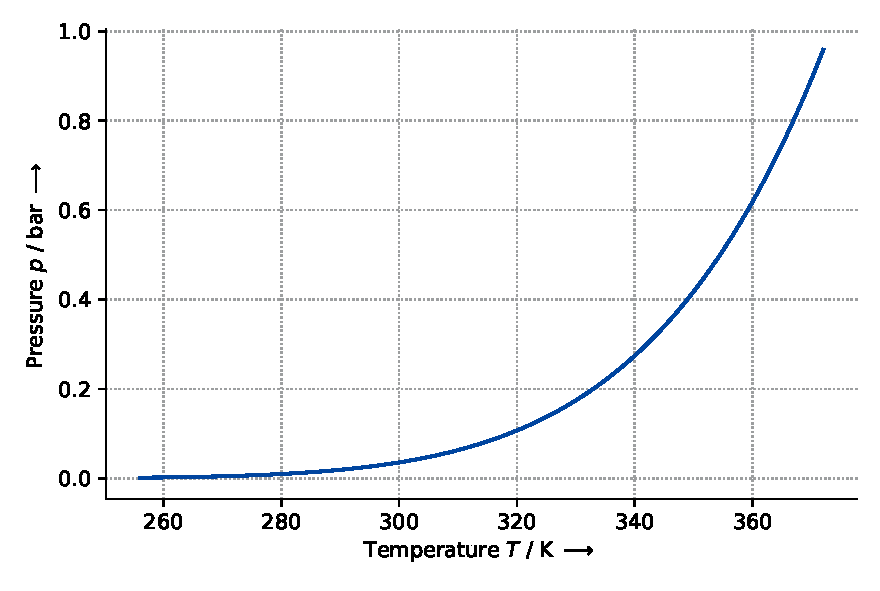
\includegraphics[height=10cm, keepaspectratio]{figs/ref/ref_Water_VaporPressure_Antoine_7.pdf}}
\end{figure}
%

\FloatBarrier
\newpage
%%%%%%%%%%%%%%%%%%%%%%%%%%%%%%%%%%%%%%%%%%%%%%%%%%%%%%%%%%%%%%%%%%%%%%%%%%%%%%%
%%%%%%%%%%%%%%%%%%%%%%%%%%%%%%%%%%%%%%%%%%%%%%%%%%%%%%%%%%%%%%%%%%%%%%%%%%%%%%%
\subsection{Vapor Pressure - EoS1 - ID 1}
%
\begin{tabular}[l]{|lp{11.5cm}|}
\hline
\addlinespace

\textbf{Name:} & Water \\
\textbf{Equation:} & VaporPressure\_EoS1 \\
\textbf{ID:} & 1 \\
\textbf{Reference:} & Wagner, W.; Pruß, A. (2002): The IAPWS Formulation 1995 for the Thermodynamic Properties of Ordinary Water Substance for General and Scientific Use. In: Journal of Physical and Chemical Reference Data 31 (2), S. 387–535. DOI: 10.1063/1.1461829. \\
\textbf{Comment:} & None \\

\addlinespace
\hline
\end{tabular}
\newline

\textbf{Equation and parameters:}
\newline
%
Vapor pressure $p_\mathrm{sat}$ in $\si{\pascal}$ is calculated depending on temperature $T$ in $\si{\kelvin}$ by:
%
\begin{equation*}
\begin{split}
p_\mathrm{sat} &=& p_\mathrm{crit} \exp \left( \nicefrac{1}{\theta} \sum_{i=1}^{7} a_i \xi^{b_i} \right) & \quad\text{, and} \\
\xi &=& 1 - \theta & \quad\text{, and} \\
\theta &=& \nicefrac{T}{T_\mathrm{crit}} & \quad\text{.}
\end{split}
\end{equation*}
%
The parameters of the equation are:
%
\begin{longtable}[l]{lll|lll}
\toprule
\addlinespace
\textbf{Par.} & \textbf{Unit} & \textbf{Value} &	\textbf{Par.} & \textbf{Unit} & \textbf{Value} \\
\addlinespace
\midrule
\endhead

\bottomrule
\endfoot
\bottomrule
\endlastfoot
\addlinespace

$T_\mathrm{crit}$ & $\si{\kelvin}$ & 6.470960000e+02 & $a_4$ & - & 2.268074110e+01 \\
$p_\mathrm{crit}$ & $\si{\pascal}$ & 2.206400000e+07 & $b_4$ & - & 3.500000000e+00 \\
$a_1$ & - & -7.859517830e+00 & $a_5$ & - & -1.596187190e+01 \\
$b_1$ & - & 1.000000000e+00 & $b_5$ & - & 4.000000000e+00 \\
$a_2$ & - & 1.844082590e+00 & $a_6$ & - & 1.801225020e+00 \\
$b_2$ & - & 1.500000000e+00 & $b_6$ & - & 7.500000000e+00 \\
$a_3$ & - & -1.178664970e+01 & $a_7$ & - & 0.000000000e+00 \\
$b_3$ & - & 3.000000000e+00 & $b_7$ & - & 0.000000000e+00 \\

\addlinespace\end{longtable}

\textbf{Validity:}
\newline
Equation is approximately valid for $273.16 \si{\kelvin} \leq T \leq 647.096 \si{\kelvin}$.
\newline

\textbf{Visualization:}
%
\begin{figure}[!htp]
{\noindent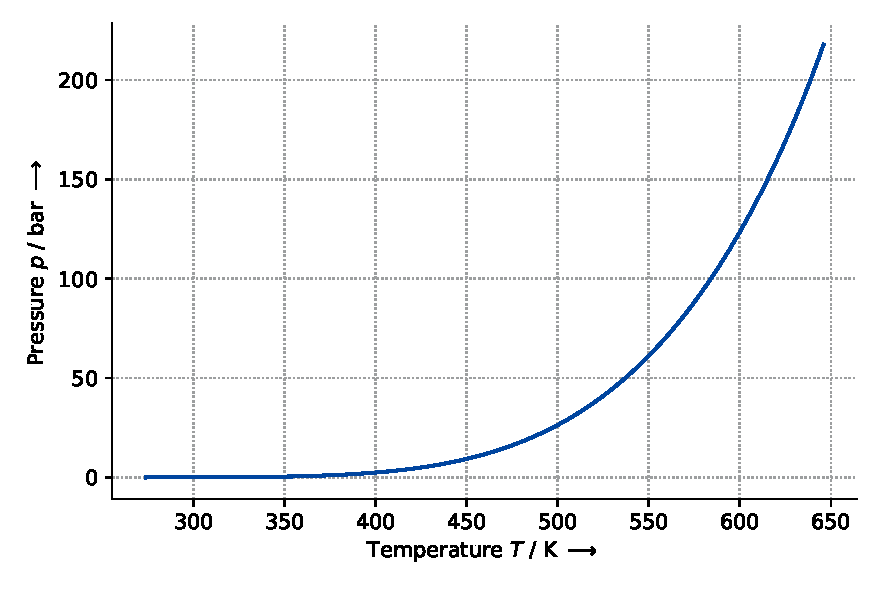
\includegraphics[height=10cm, keepaspectratio]{figs/ref/ref_Water_VaporPressure_EoS1_1.pdf}}
\end{figure}
%

\FloatBarrier
\newpage
%%%%%%%%%%%%%%%%%%%%%%%%%%%%%%%%%%%%%%%%%%%%%%%%%%%%%%%%%%%%%%%%%%%%%%%%%%%%%%%
%%%%%%%%%%%%%%%%%%%%%%%%%%%%%%%%%%%%%%%%%%%%%%%%%%%%%%%%%%%%%%%%%%%%%%%%%%%%%%%
\subsection{Vapor Pressure - EoS1 - ID 2}
%
\begin{tabular}[l]{|lp{11.5cm}|}
\hline
\addlinespace

\textbf{Name:} & Water \\
\textbf{Equation:} & VaporPressure\_EoS1 \\
\textbf{ID:} & 2 \\
\textbf{Reference:} & Verein Deutscher Ingenieure (2010): VDI Heat Atlas. 2. Ed. Heidelberg: Springer. Online: http://dx.doi.org/10.1007/978-3-540-77877-6. \\
\textbf{Comment:} & None \\

\addlinespace
\hline
\end{tabular}
\newline

\textbf{Equation and parameters:}
\newline
%
Vapor pressure $p_\mathrm{sat}$ in $\si{\pascal}$ is calculated depending on temperature $T$ in $\si{\kelvin}$ by:
%
\begin{equation*}
\begin{split}
p_\mathrm{sat} &=& p_\mathrm{crit} \exp \left( \nicefrac{1}{\theta} \sum_{i=1}^{7} a_i \xi^{b_i} \right) & \quad\text{, and} \\
\xi &=& 1 - \theta & \quad\text{, and} \\
\theta &=& \nicefrac{T}{T_\mathrm{crit}} & \quad\text{.}
\end{split}
\end{equation*}
%
The parameters of the equation are:
%
\begin{longtable}[l]{lll|lll}
\toprule
\addlinespace
\textbf{Par.} & \textbf{Unit} & \textbf{Value} &	\textbf{Par.} & \textbf{Unit} & \textbf{Value} \\
\addlinespace
\midrule
\endhead

\bottomrule
\endfoot
\bottomrule
\endlastfoot
\addlinespace

$T_\mathrm{crit}$ & $\si{\kelvin}$ & 6.471000000e+02 & $a_4$ & - & -2.064720000e+00 \\
$p_\mathrm{crit}$ & $\si{\pascal}$ & 2.206400000e+07 & $b_4$ & - & 5.000000000e+00 \\
$a_1$ & - & -7.869750000e+00 & $a_5$ & - & 0.000000000e+00 \\
$b_1$ & - & 1.000000000e+00 & $b_5$ & - & 0.000000000e+00 \\
$a_2$ & - & 1.905610000e+00 & $a_6$ & - & 0.000000000e+00 \\
$b_2$ & - & 1.500000000e+00 & $b_6$ & - & 0.000000000e+00 \\
$a_3$ & - & -2.308910000e+00 & $a_7$ & - & 0.000000000e+00 \\
$b_3$ & - & 2.500000000e+00 & $b_7$ & - & 0.000000000e+00 \\

\addlinespace\end{longtable}

\textbf{Validity:}
\newline
Equation is approximately valid for $273.16 \si{\kelvin} \leq T \leq 647.1 \si{\kelvin}$.
\newline

\textbf{Visualization:}
%
\begin{figure}[!htp]
{\noindent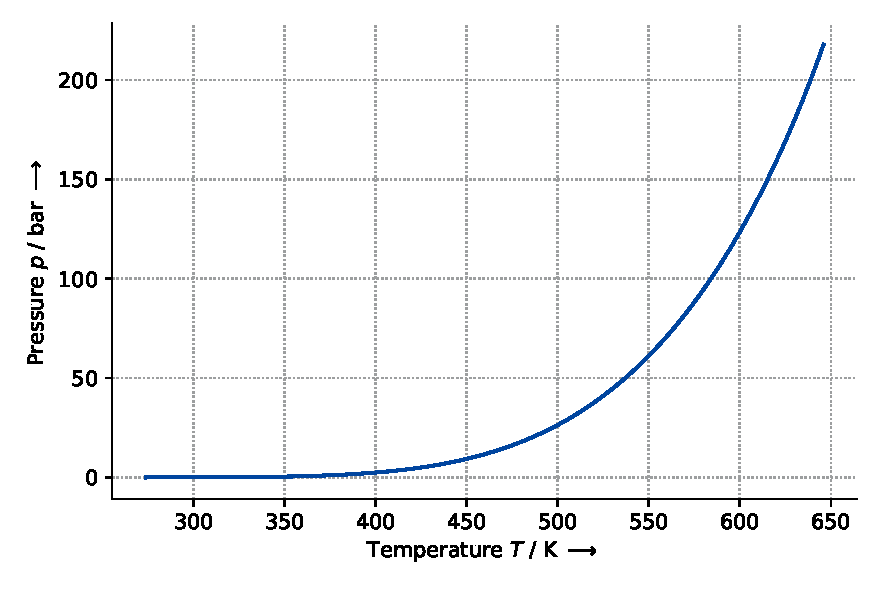
\includegraphics[height=10cm, keepaspectratio]{figs/ref/ref_Water_VaporPressure_EoS1_2.pdf}}
\end{figure}
%

\FloatBarrier
\newpage
%%%%%%%%%%%%%%%%%%%%%%%%%%%%%%%%%%%%%%%%%%%%%%%%%%%%%%%%%%%%%%%%%%%%%%%%%%%%%%%
%%%%%%%%%%%%%%%%%%%%%%%%%%%%%%%%%%%%%%%%%%%%%%%%%%%%%%%%%%%%%%%%%%%%%%%%%%%%%%%
\subsection{Vapor Pressure - EoSCubic - ID 1}
%
\begin{tabular}[l]{|lp{11.5cm}|}
\hline
\addlinespace

\textbf{Name:} & Water \\
\textbf{Equation:} & VaporPressure\_EoSCubic \\
\textbf{ID:} & 1 \\
\textbf{Reference:} & Lemmon, E. W.; Bell, I. H.; Huber, M. L.; McLinden, M. O. (2018): NIST Standard Reference Database 23. Reference Fluid Thermodynamic and Transport Properties-REFPROP, Version 10.0, National Institute of Standards and Technology. Online: https://www.nist.gov/srd/refprop. \\
\textbf{Comment:} & None \\

\addlinespace
\hline
\end{tabular}
\newline

\textbf{Equation and parameters:}
\newline
%
Vapor pressure $p_\mathrm{sat}$ in $\si{\pascal}$ is calculated depending on temperature $T$ in $\si{\kelvin}$ and molar volume v in $\si{\mole\per\cubic\meter}$ by using cubic equation of state. For this purpose, molar volumes of liquid and vapor phase are changed iteratively until fugacity coefficients of vapor and liquid phase are equal. Cubic equation of state is given by:
\begin{equation*}
\begin{split}
p &=& R \frac{T}{v - b} - \frac{a}{v \left(v + b\right)} & \quad\text{, and} \\
a &=& \frac{1}{9 \left(2^{\nicefrac{1}{3}} - 1\right)} \frac{\left(R T_\mathrm{crit} \right)^2}{p_\mathrm{crit}} \alpha & \quad\text{, and} \\
b &=& 0.08664 R \frac{T_\mathrm{crit}}{p_\mathrm{crit}} & \quad\text{, and} \\
\alpha &=& \left(1 + \kappa \left(1 - \sqrt(\nicefrac{T}{T_\mathrm{crit}}) \right) \right)^2 & \quad\text{, and} \\
\kappa &=& 0.48508 + 1.55171 \omega - 0.15613 \omega^2 & \quad\text{.}
\end{split}
\end{equation*}
%
The parameters of the equation are:
%
\begin{longtable}[l]{lll|lll}
\toprule
\addlinespace
\textbf{Par.} & \textbf{Unit} & \textbf{Value} &	\textbf{Par.} & \textbf{Unit} & \textbf{Value} \\
\addlinespace
\midrule
\endhead

\bottomrule
\endfoot
\bottomrule
\endlastfoot
\addlinespace

EoS & - & -5.000000000e+00 & $\beta_0$ & - & 0.000000000e+00 \\
$T_\mathrm{crit}$ & $\si{\kelvin}$ & 6.471000000e+02 & $\beta_1$ & - & 0.000000000e+00 \\
$p_\mathrm{crit}$ & $\si{\pascal}$ & 2.206400000e+07 & $\beta_2$ & - & 0.000000000e+00 \\
$\omega$ & - & 3.443000000e-01 & $\beta_3$ & - & 0.000000000e+00 \\
$\kappa_1$ & - & 0.000000000e+00 & & & \\

\addlinespace\end{longtable}

\textbf{Validity:}
\newline
Equation is approximately valid for $314.134 \si{\kelvin} \leq T \leq 550.035 \si{\kelvin}$.
\newline

\textbf{Visualization:}
%
\begin{figure}[!htp]
{\noindent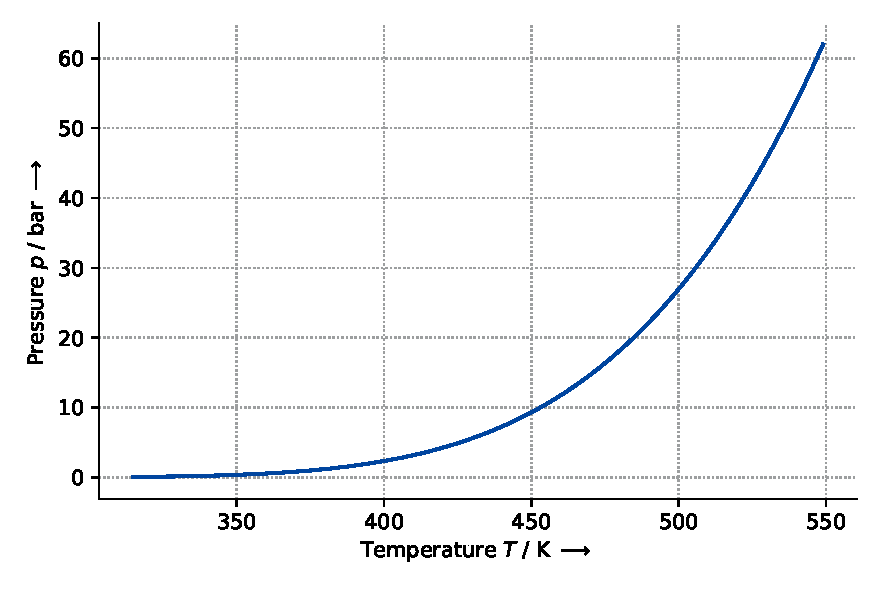
\includegraphics[height=10cm, keepaspectratio]{figs/ref/ref_Water_VaporPressure_EoSCubic_1.pdf}}
\end{figure}
%

\FloatBarrier
\newpage
%%%%%%%%%%%%%%%%%%%%%%%%%%%%%%%%%%%%%%%%%%%%%%%%%%%%%%%%%%%%%%%%%%%%%%%%%%%%%%%
%%%%%%%%%%%%%%%%%%%%%%%%%%%%%%%%%%%%%%%%%%%%%%%%%%%%%%%%%%%%%%%%%%%%%%%%%%%%%%%
\subsection{Vapor Pressure - EoSCubic - ID 2}
%
\begin{tabular}[l]{|lp{11.5cm}|}
\hline
\addlinespace

\textbf{Name:} & Water \\
\textbf{Equation:} & VaporPressure\_EoSCubic \\
\textbf{ID:} & 2 \\
\textbf{Reference:} & Lemmon, E. W.; Bell, I. H.; Huber, M. L.; McLinden, M. O. (2018): NIST Standard Reference Database 23. Reference Fluid Thermodynamic and Transport Properties-REFPROP, Version 10.0, National Institute of Standards and Technology. Online: https://www.nist.gov/srd/refprop. \\
\textbf{Comment:} & None \\

\addlinespace
\hline
\end{tabular}
\newline

\textbf{Equation and parameters:}
\newline
%
Vapor pressure $p_\mathrm{sat}$ in $\si{\pascal}$ is calculated depending on temperature $T$ in $\si{\kelvin}$ and molar volume v in $\si{\mole\per\cubic\meter}$ by using cubic equation of state. For this purpose, molar volumes of liquid and vapor phase are changed iteratively until fugacity coefficients of vapor and liquid phase are equal. Cubic equation of state is given by:
\begin{equation*}
\begin{split}
p &=& R \frac{T}{v - b} - \frac{a}{v \left(v + b\right) + b \left(v - b\right)} & \quad\text{, and} \\
a &=& 0.45724 \frac{\left(R T_\mathrm{crit} \right)^2}{p_\mathrm{crit}} \alpha & \quad\text{, and} \\
b &=& 0.07780 R \frac{T_\mathrm{crit}}{p_\mathrm{crit}} & \quad\text{, and} \\
\alpha &=& \left(1 + \kappa \left(1 - \sqrt(\nicefrac{T}{T_\mathrm{crit}}) \right) \right)^2 & \quad\text{, and} \\
\kappa &=& 0.37464 + 1.54226 \omega - 0.26992 \omega^2 & \quad\text{.}
\end{split}
\end{equation*}
%
The parameters of the equation are:
%
\begin{longtable}[l]{lll|lll}
\toprule
\addlinespace
\textbf{Par.} & \textbf{Unit} & \textbf{Value} &	\textbf{Par.} & \textbf{Unit} & \textbf{Value} \\
\addlinespace
\midrule
\endhead

\bottomrule
\endfoot
\bottomrule
\endlastfoot
\addlinespace

EoS & - & 1.000000000e+01 & $\beta_0$ & - & 0.000000000e+00 \\
$T_\mathrm{crit}$ & $\si{\kelvin}$ & 6.471000000e+02 & $\beta_1$ & - & 0.000000000e+00 \\
$p_\mathrm{crit}$ & $\si{\pascal}$ & 2.206400000e+07 & $\beta_2$ & - & 0.000000000e+00 \\
$\omega$ & - & 3.443000000e-01 & $\beta_3$ & - & 0.000000000e+00 \\
$\kappa_1$ & - & 0.000000000e+00 & & & \\

\addlinespace\end{longtable}

\textbf{Validity:}
\newline
Equation is approximately valid for $314.134 \si{\kelvin} \leq T \leq 550.035 \si{\kelvin}$.
\newline

\textbf{Visualization:}
%
\begin{figure}[!htp]
{\noindent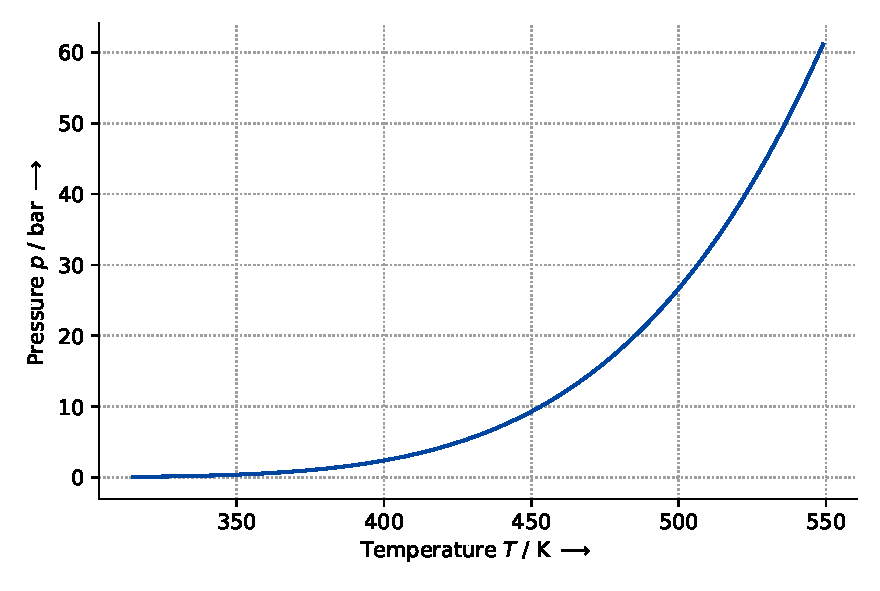
\includegraphics[height=10cm, keepaspectratio]{figs/ref/ref_Water_VaporPressure_EoSCubic_2.pdf}}
\end{figure}
%

\FloatBarrier
\newpage
%%%%%%%%%%%%%%%%%%%%%%%%%%%%%%%%%%%%%%%%%%%%%%%%%%%%%%%%%%%%%%%%%%%%%%%%%%%%%%%
